\chapter{量子コンピュータ: 物理的実現方法}

\begin{ex}
    \label{ex7.1}
    \begin{align*}
        a^\dagger a
        =
        \frac{1}{2m\hbar \omega}
        \left( m^2 \omega^2 x^2 + p^2 + i m\omega \left[x,p\right] \right)
        =
        \frac{1}{\hbar \omega}
        \left(  \frac{p^2}{2m} + \frac{m \omega^2 x^2}{2} \right) - \frac{1}{2}.
    \end{align*}
\end{ex}

\begin{ex}
    \label{ex7.2}
    \begin{align*}
        \left[a, a^\dagger\right]
        =
        \frac{-2i m \omega \left[x,p\right] }{2m\hbar \omega}
        =
        1.
    \end{align*}
\end{ex}

\begin{ex}
    \label{ex7.3}
    \begin{align*}
        \left[H,a\right]
        = \left[ \hbar \omega a^\dagger a, a\right]
        = \hbar \omega [a^\dagger ,a]a
        = - \hbar \omega a
    \end{align*}
    であるので,
    \begin{align*}
        H \ket{\psi} = E \ket{\psi}
    \end{align*}
    なる$\ket{\psi}$に対して,
    \begin{align*}
        E a \ket{\psi} = aH \ket{\psi} = \left(Ha + \hbar \omega a \right) \ket{\psi}
        \to
        H a\ket{\psi} = \left(E - \hbar \omega \right) a \ket{\psi}
    \end{align*}
    を得る. これを帰納的に繰り返して,
    \begin{align*}
        H a^n \ket{\psi} = \left( E - nh\omega\right) \ket{\psi}.
    \end{align*}
\end{ex}

\begin{ex}
    \label{ex7.4}
    式(7.11);
    \begin{align*}
        a^\dagger \ket{n} = \sqrt{n+1} \ket{n+1}
    \end{align*}
    より,
    \begin{align*}
        \left(a^\dagger \right)^n \ket{0} = \sqrt{n!} \ket{n}.
    \end{align*}
\end{ex}

\begin{ex}
    \label{ex7.5}
    式(7.10), 正規化条件, $\left[a,a^\dagger\right] = 1$より,
    \begin{align*}
        \left| a^\dagger \ket{n}\right|^2 & = \braket{n|aa^\dagger|n} =
        \braket{n|a^\dagger a + 1|n} = n+1
        \\
        \left| a \ket{n}\right|^2         & = \braket{n|a^\dagger a|n} = n
    \end{align*}
\end{ex}

\begin{ex}
    \label{ex7.6}
    \begin{align*}
        a \ket{\alpha}
        =
        e^{-\frac{|\alpha|^2}{2}} \sum_{n=0}^\infty \frac{\alpha^n}{\sqrt{n!}} a \ket{n}
        =
        e^{-\frac{|\alpha|^2}{2}} \sum_{n=1}^\infty \frac{\alpha^n}{\sqrt{(n-1)!}}  \ket{n-1}
        =
        \alpha
        e^{-\frac{|\alpha|^2}{2}} \sum_{n=1}^\infty \frac{\alpha^{n-1}}{\sqrt{(n-1)!}}  \ket{n-1}
        =
        \alpha \ket{\alpha}
    \end{align*}
\end{ex}

\begin{ex}
    \label{ex7.7}
    明らか.
\end{ex}

\begin{ex}
    \label{ex7.8}
    Kerr物質を用いた位相シフタ$P$は, 系の光子の数に比例した分だけ位相をズラすオペレータ;
    \begin{align*}
        P\ket{n} = e^{i \Delta n} \ket{n}
    \end{align*}
    なので,
    \begin{align*}
        P \ket{\alpha}
        =
        e^{-\frac{|\alpha|^2}{2}}
        \sum_{n=0}^\infty \frac{\alpha^n}{\sqrt{n!}}e^{i \Delta n} \ket{n}
        =
        e^{-\frac{\left|\alpha e^{i \Delta} \right|^2}{2}}
        \sum_{n=0}^\infty \frac{ \left( {\alpha e^{i \Delta }}\right)^n}{\sqrt{n!}} \ket{n}
        =
        \ket{\alpha e^{i\Delta}}.
    \end{align*}
\end{ex}

\begin{ex}
    \label{ex7.9}
    $\theta = \pi / 4$のビームスプリッタ$B$を考えると,
    \begin{align*}
        e^{i \pi} B\ket{01} = - \frac{\ket{01} + \ket{10}}{\sqrt{2}} \\
        B \ket{10} = \frac{\ket{11} - \ket{01}}{\sqrt{2}}
    \end{align*}
    となり, 全体の位相をのぞいてHadamard変換になっている.
\end{ex}

\begin{ex}
    \label{ex7.10}
    行列表示で,
    \begin{align*}
        \begin{pmatrix}
            \cos \beta & \sin \beta \\
            -\sin\beta & \cos \beta
        \end{pmatrix}
        \begin{pmatrix}
            e^{i\phi} & 0 \\
            0         & 1
        \end{pmatrix}
        \begin{pmatrix}
            \cos \alpha & -\sin\alpha \\
            \sin \alpha & \cos \alpha
        \end{pmatrix}
        =
        e^{\frac{i \phi}{2}}
        R_y(-2\beta) R_z(-\phi) R_y(2\alpha)
    \end{align*}
\end{ex}

\begin{ex}
    \label{ex7.11}
    \begin{align*}
        B \ket{20}
         & =
        \frac{1}{\sqrt{2}}Bb^\dagger b^\dagger \ket{00}                                                                   \\
         & =
        \frac{1}{\sqrt{2}}Bb^\dagger B^\dagger B b^\dagger B^\dagger B \ket{00}                                           \\
         & =
        \frac{1}{\sqrt{2}}\frac{-a^\dagger + b^\dagger}{\sqrt{2}}\frac{-a^\dagger + b^\dagger}{\sqrt{2}}\ket{00}          \\
         & =
        \frac{a^\dagger a^\dagger - b^\dagger a^\dagger - a^\dagger b^\dagger + b^\dagger b^\dagger}{2 \sqrt{2}} \ket{00} \\
         & =
        \frac{1}{{2}}\ket{02} - \frac{1}{\sqrt{2}}\ket{11} + \frac{1}{{2}}\ket{20}.
    \end{align*}
\end{ex}

\begin{ex}
    \label{ex7.12}
    $b^\dagger \otimes I$や$I \otimes a^\dagger$を単に$b^\dagger$や$a^\dagger$とかく.
    \begin{align*}
        B \ket{\alpha}\otimes\ket{\beta}
         & =
        Be^{- \left(|\alpha|^2 + |\beta|^2 \right)}
        \sum_{n,m}\frac{\alpha^n \beta^m}{ \sqrt{n! m!}} \ket{n} \otimes \ket{m}
        \\
         & =
        Be^{- \left(|\alpha|^2 + |\beta|^2 \right)}
        \sum_{n,m}\frac{\alpha^n \beta^m}{ {n! m!}} \left(b^\dagger\right)^n
        \left(a^\dagger\right)^m \ket{0} \otimes \ket{0}
        \\
         & =
        e^{- \left(|\alpha|^2 + |\beta|^2 \right)}
        \sum_{n,m}\frac{\alpha^n \beta^m}{ {n! m!}}
        \left(B b^\dagger B^\dagger \right)^n
        \left(B a^\dagger B^\dagger \right)^m
        B \ket{0} \otimes \ket{0}
        \\
         & =
        e^{- \left(|\alpha|^2 + |\beta|^2 \right)}
        \sum_{n,m}\frac{\alpha^n \beta^m}{ {n! m!}}
        \left( -a^\dagger \sin\theta + b^\dagger \cos\theta \right)^n
        \left( a^\dagger \cos\theta + b^\dagger \sin\theta\right)^m
        \ket{0} \otimes \ket{0}
        \\
         & =
        e^{- \left(|\alpha|^2 + |\beta|^2 \right)}
        \sum_{n}\frac{\alpha^n}{ n!}
        \left( -a^\dagger \sin\theta + b^\dagger \cos\theta \right)^n
        \sum_{m}\frac{\beta^m}{m!}
        \left( a^\dagger \cos\theta + b^\dagger \sin\theta\right)^m
        \ket{0} \otimes \ket{0}
        \\
         & =
        e^{- \left(|\alpha|^2 + |\beta|^2 \right)}
        \exp \left[ \left(-a^\dagger \sin\theta + b^\dagger \cos\theta  \right) \alpha
            +
            \left( a^\dagger \cos\theta + b^\dagger \sin\theta\right) \beta\right]
        \ket{0} \otimes \ket{0}
        \\
         & =
        e^{- \left(|\beta\sin\theta + \alpha \cos\theta|^2 + |\beta\cos\theta - \alpha \sin\theta|^2 \right)}
        \exp
        \left[ \left(\beta \sin\theta + \alpha \cos\theta  \right) b^\dagger
            +
            \left( \beta \cos\theta - \alpha \sin\theta\right) a^\dagger
            \right]
        \ket{0} \otimes \ket{0}
        \\
         & =
        \ket{\beta \sin\theta + \alpha \cos\theta}
        \otimes
        \ket{\beta \cos\theta - \alpha \sin\theta}.
    \end{align*}

\end{ex}

\begin{ex}
    \label{ex7.13}

\end{ex}

\begin{ex}
    \label{ex7.14}
    $b^\dagger \otimes I$や$I \otimes a^\dagger$を単に$b^\dagger$や$a^\dagger$とかく.
    \begin{align*}
        K \ket{\alpha}\ket{n}
         & =
        e^{i \chi L a^\dagger a  b^\dagger b} e^{- \frac{|\alpha|^2}{2}} \sum_m \frac{\alpha^m}{\sqrt{m!}} \ket{m} \ket{n}
        \\
         & =
        e^{i \chi L n b^\dagger b} e^{- \frac{|\alpha|^2}{2}} \sum_m \frac{\alpha^m}{\sqrt{m!}} \ket{m} \ket{n}
        \\
         & =
        e^{- \frac{|\alpha|^2}{2}}
        \sum_{m,l} \frac{1}{l!} \left(i \chi L n b^\dagger b \right)^l
        \frac{\alpha^m}{\sqrt{m!}} \ket{m} \ket{n}
        \\
         & =
        e^{- \frac{|\alpha|^2}{2}}
        \sum_{m,l} \frac{1}{l!} \left(i \chi L n m \right)^l
        \frac{\alpha^m}{\sqrt{m!}} \ket{m} \ket{n}
        \\
         & =
        e^{- \frac{\left|\alpha e^{i \chi L n} \right|^2}{2}}
        \sum_{m}
        \frac{ ( \alpha e^{i \chi L n} )^m}{\sqrt{m!}} \ket{m} \ket{n}
        \\
         & =\ket{\alpha e^{i \chi L n}} \ket{n}
    \end{align*}
    なので,
    \begin{align*}
        K \ket{\alpha}\ket{\beta}
         & =
        K e^{-\frac{|\beta|^2}{2}} \sum_n \frac{\beta^n}{\sqrt{n!}} \ket{\alpha}\ket{n}
        \\
         & =
        e^{-\frac{|\beta|^2}{2}} \sum_n \frac{\beta^n}{\sqrt{n!}} \ket{\alpha e^{i\chi L n}}\ket{n}
    \end{align*}
    であることから,
    \begin{align*}
        \rho_a
         & =
        \tr_b \left[ K \ket{\alpha}\ket{\beta} \bra{\beta} \bra{\alpha} K^\dagger\right] \\
         & =
        e^{- |\beta|^2}
        \tr_b \left[
            \sum_{n,m}
            \frac{\beta^n}{\sqrt{n!}} \frac{\bar{\beta}^m}{\sqrt{m!}}
            \ket{\alpha e^{i\chi L n}}\ket{n} \bra{m} \bra{\alpha e^{i\chi L m}}
            \right]
        \\
         & =
        e^{- |\beta|^2}
        \tr_b \left[
            \sum_{n,m}
            \delta_{nm}
            \frac{\beta^n}{\sqrt{n!}} \frac{\bar{\beta}^m}{\sqrt{m!}}
            \ket{\alpha e^{i\chi L n}} \bra{\alpha e^{i\chi L m}}
            \right]
        \\
         & =
        e^{- |\beta|^2}
        \sum_{n}
        \frac{\left| \beta \right|^{2n}}{n!}
        \ket{\alpha e^{i\chi L n}} \bra{\alpha e^{i\chi L n}}
    \end{align*}
    を得る. この和の主な寄与をもたらす$n$は,
    \begin{align*}
        1 = \frac{|\beta|^{2(n-1)}}{(n-1)!} \frac{n!}{|\beta|^{2n}} \to n \sim |\beta|^2.
    \end{align*}
\end{ex}

\begin{ex}
    \label{ex7.15}
    \
    \begin{figure}[H]
        \begin{center}
            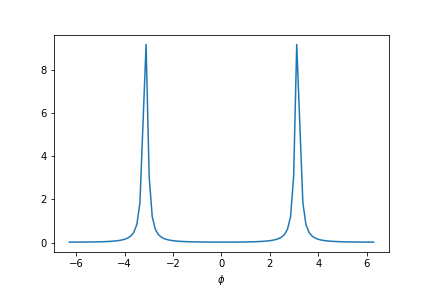
\includegraphics[width = 80mm]{../fig/ex7_15.png}
        \end{center}
    \end{figure}
\end{ex}

\begin{ex}
    \label{ex7.16}
    $m=\pm1$とする.
    \begin{align*}
        I \equiv \int Y_{l_1,m_1}^* Y_{1,m} Y_{l_2,m_2} d\Omega
         & \propto
        \int_{0}^\pi P_{l_1,m_1}(\cos \theta) \sin\theta P_{l_2,m_2}(\cos \theta) \ d\cos\theta
        \int_{0}^{2\pi} e^{i(-m_1+m+m_2)\phi}\ d\phi.
    \end{align*}
    $I$の$\phi$成分の積分に注目すると, $I \neq 0$であるためには,
    \begin{align*}
        \int_{0}^{2\pi} e^{i(-m_1+m+m_2)\phi}\ d\phi \neq 0
        \longleftrightarrow
        -m_1 + m + m_2 = 0
        \longleftrightarrow
        m_1 - m_2 = m = \pm1
    \end{align*}
    であることが必要.
    \par
    以下では$m=1$の場合だけ考えるが, $m=-1$の場合も同様である. 先の条件より,
    \begin{align*}
        m_1 = m_2 +1.
    \end{align*}
    Legendre陪多項式についての漸化式
    \begin{align*}
        \sin\theta P_{m,l}(\cos\theta)
        = \frac{1}{2l +1}\left[P_{l+1,m+1}(\cos \theta) - P_{l-1,m+1}(\cos\theta)\right]
    \end{align*}
    を用いて, $I$の$\theta$成分の積分は,
    \begin{align*}
           & \int_{0}^\pi P_{l_1,m_2 + 1}(\cos \theta) \sin\theta P_{l_2,m_2}(\cos \theta) \ d\cos\theta \\
        \  & =
        \frac{1}{2 l_2 + 1}\int_{0}^\pi P_{l_1,m_2+1}(\cos \theta)
        \left[P_{l_2+1,m_2+1}(\cos \theta) - P_{l_2-1,m_2+1}(\cos\theta)\right]
        \ d\cos\theta                                                                                    \\
    \end{align*}
    となる. よって, Legendre陪多項式の直交性より, $m=1$の時, $I$の$\theta$成分の積分が$0$にならないための必要十分条件は, $m_1 - m_2 = 1$かつ$l_1 = l_2 \pm 1$.
    \par
    以上より,
    \begin{align*}
        I \neq 0 \longleftrightarrow m_1 - m_2 = \pm 1 \mathrm{かつ} l_1 - l_2 = \pm1.
    \end{align*}
\end{ex}

\begin{ex}
    \label{ex7.17}
    $\omega = \delta = 0$のとき, Jaynes-CummingsのHamiltonian$H$は,
    \begin{align*}
        H = g \left( a^\dagger \sigma_- + a \sigma_+\right).
    \end{align*}
    よって,
    \begin{align*}
        H\ket{\chi_n}
         & =
        g \left( a^\dagger \sigma_- + a \sigma_+\right) \frac{\ket{n,1} + \ket{n+1, 0}}{\sqrt{2}}
        =
        g \frac{ \sqrt{n+1} \ket{n+1,0} + \sqrt{n+1}\ket{n, 1}}{\sqrt{2}}
        =
        g\sqrt{n+1}\ket{\chi_n}
        \\
        H\ket{\bar{\chi}_n}
         & =
        g \left( a^\dagger \sigma_- + a \sigma_+\right) \frac{\ket{n,1} - \ket{n+1, 0}}{\sqrt{2}}
        =
        g \frac{ \sqrt{n+1} \ket{n+1,0} - \sqrt{n+1}\ket{n, 1}}{\sqrt{2}}
        =
        -g\sqrt{n+1}\ket{\bar{\chi}_n}.
    \end{align*}
\end{ex}

\begin{ex}
    \label{ex7.18}
    時間発展演算子$U$は, $\Omega = \sqrt{g^2 + \delta^2}$を用いて,
    \begin{align*}
        U & =
        \exp \left[ - i H t \right]
        \\
          & =
        e^{ i \delta t } \ket{00}\bra{00}
        +
        \exp \left[
            i
            \begin{pmatrix}
                - \delta t & g t      \\
                gt         & \delta t
            \end{pmatrix}
            \right] \\
          & =
        e^{ i \delta t } \ket{00}\bra{00}+
        \exp \left[
            igt X - i\delta t Z
            \right] \\
          & =
        e^{ i \delta t } \ket{00}\bra{00}+
        I \cos \Omega t + i \frac{g}{\Omega} X \sin \Omega t - i \frac{\delta}{\Omega} Z \sin \Omega t
        \\
          & =
        e^{ i \delta t } \ket{00}\bra{00}+
        \left( \ket{01} \bra{01} + \ket{10}\bra{10}\right)\cos \Omega t
        + i \frac{g}{\Omega} \sin \Omega t  \left( \ket{01}\bra{10} + \ket{10}\ket{01}\right)
        - i \frac{\delta}{\Omega} \sin \Omega t \left( \ket{01} \bra{01} -\ket{10}\bra{10}\right)
        \\
          & =
        e^{ i \delta t } \ket{00}\bra{00}+
        \left( \cos \Omega t + i \frac{\delta}{\Omega} \sin\Omega t\right) \ket{01}\bra{01}
        +
        \left( \cos \Omega t + i \frac{\delta}{\Omega} \sin\Omega t\right) \ket{10}\bra{10}
        -
        i \frac{g}{\Omega} \sin\Omega t \left( \ket{01}\bra{10} + \ket{10}\bra{01}\right).
    \end{align*}
\end{ex}

\begin{ex}
    \label{ex7.19}
    \
    \begin{figure}[H]
        \begin{center}
            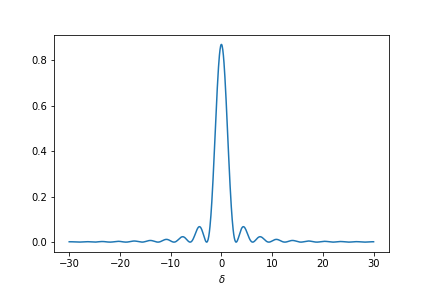
\includegraphics[width = 80mm]{../fig/ex7_19.png}
        \end{center}
    \end{figure}
\end{ex}

\begin{ex}
    \label{ex7.20}
    \
    \begin{figure}[H]
        \begin{center}
            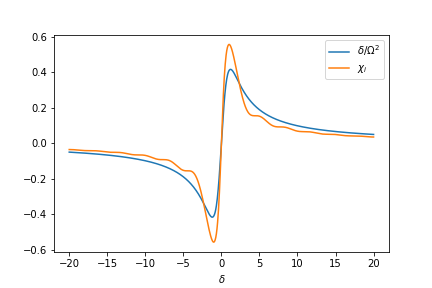
\includegraphics[width = 80mm]{../fig/ex7_20.png}
        \end{center}
    \end{figure}
\end{ex}

\begin{ex}
    \label{ex7.21}
    $\arg(\braket{110|U|110})$を求めるには, $U = \exp\left[ - i H t\right]$の$\ket{110}\bra{110}$成分だけ考えればよい. すると,
    \begin{align*}
        H_2^n
        =
        \begin{pmatrix}
            -\delta & g_a    & g_b    \\
            g_a     & \delta & 0      \\
            g_b     & 0      & \delta
        \end{pmatrix}^n
        =
        \begin{cases}
            \Omega'^{n} \ket{110}\bra{110} + ...\             & (n \mathrm{\ is\ even}) \\
            - \delta \Omega'^{n-1} \ket{110}\bra{110} + ...\  & (n \mathrm{\ is\ odd})
        \end{cases}
    \end{align*}
    なので,
    \begin{align*}
        \braket{110|U|110}
         & =
        \braket{110|\exp\left[ - i H t\right]|110}
        \\
         & =
        \braket{110|\exp\left[ - i H_2 t\right]|110}
        \\
         & =
        \braket{ 110|\sum_n \frac{1}{n!} (-i H_2 t)^n |110}
        \\
         & =
        \sum_{\mathrm{n\ is \ even}}
        \frac{(-1)^\frac{n}{2} t^n}{n!}
        \Omega'^{n}
        + i \delta
        \sum_{\mathrm{n\ is \ odd}}
        \frac{(-1)^\frac{n-1}{2} t^{n}}{n!}
        \Omega'^{n-1}
        \\
         & =
        \sum_{n}
        \frac{(-1)^n t^{2n}}{(2n)!}
        \Omega'^{2n}
        + i
        \frac{\delta}{\Omega'}
        \sum_{n}
        \frac{(-1)^n t^{2n+1}}{(2n+1)!}
        \Omega'^{2n+1}
        \\
         & =
        \cos\Omega' t + i \frac{\delta}{\Omega'} \sin\Omega't
    \end{align*}
    を得る. よって,
    \begin{align*}
        \phi_{ab} = \arg(\braket{110|U|110}) - \arg(\braket{000|U|000})
         & =\arg\left(\cos\Omega' t + i \frac{\delta}{\Omega'} \sin\Omega't \right) - \arg\left(e^{i \delta t}\right) \\
         & =
        \arg\left[\left(\cos\Omega' t + i \frac{\delta}{\Omega'} \sin\Omega't \right)e^{- i \delta t} \right].
    \end{align*}
    $\phi_a, \phi_b$については, $\Omega_i = \sqrt{g_i^2 + \delta^2}$として, 式(7.77)と全く同様の計算をして,
    \begin{align*}
        \phi_a
         & = \arg\left( \braket{100|U|100}\right) - \arg\left( \braket{000|U|000}\right)
        =  \arg\left[ \left(\cos\Omega_a t - i \frac{\delta}{\Omega_a} \sin\Omega_a t\right) e^{- i \delta t} \right]
        \\
        \phi_b
         & = \arg\left( \braket{010|U|010}\right) - \arg\left( \braket{010|U|010}\right)
        =  \arg\left[
        \left(\cos\Omega_b t - i \frac{\delta}{\Omega_b} \sin\Omega_b t \right)e^{- i \delta t} \right]
    \end{align*}
    \par
    以上より,
    \begin{align*}
        \chi_3 = \phi_{ab} - \phi_a - \phi_b
        =
        \arg\left[
            \frac{\cos\Omega' t + i \frac{\delta}{\Omega'} \sin\Omega't }
            {\left(\cos\Omega_a t - i \frac{\delta}{\Omega_a} \sin\Omega_a t\right)
                \left(\cos\Omega_b t - i \frac{\delta}{\Omega_b} \sin\Omega_b t \right)}
            e^{i \delta t}
            \right]
    \end{align*}
    $\chi_3$の$\delta$依存性を図示すると, 以下のようになる.
    \begin{figure}[H]
        \begin{center}
            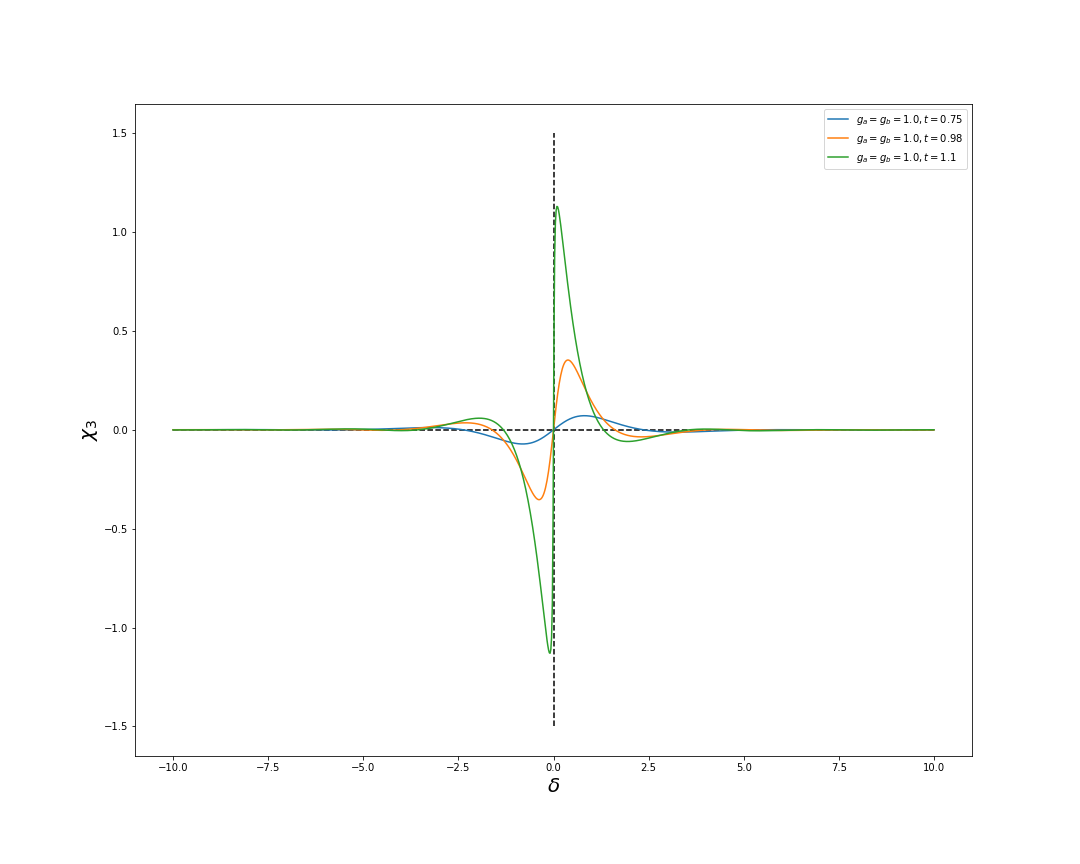
\includegraphics[width = 100mm]{../fig/ex7_21.png}
        \end{center}
    \end{figure}
\end{ex}

\begin{ex}
    \label{ex7.22}
    演習\ref{ex7.21}より, 光子が原子に吸収される確率は,
    \begin{align*}
        1 - \left| \braket{110|U|110}\right|^2
        =  1 - \left(\cos\Omega' t\right)^2 - \left(\frac{\delta}{\Omega'} \sin\Omega't \right)^2
    \end{align*}
    図示すると, 以下のようになる.
    \begin{figure}[H]
        \begin{center}
            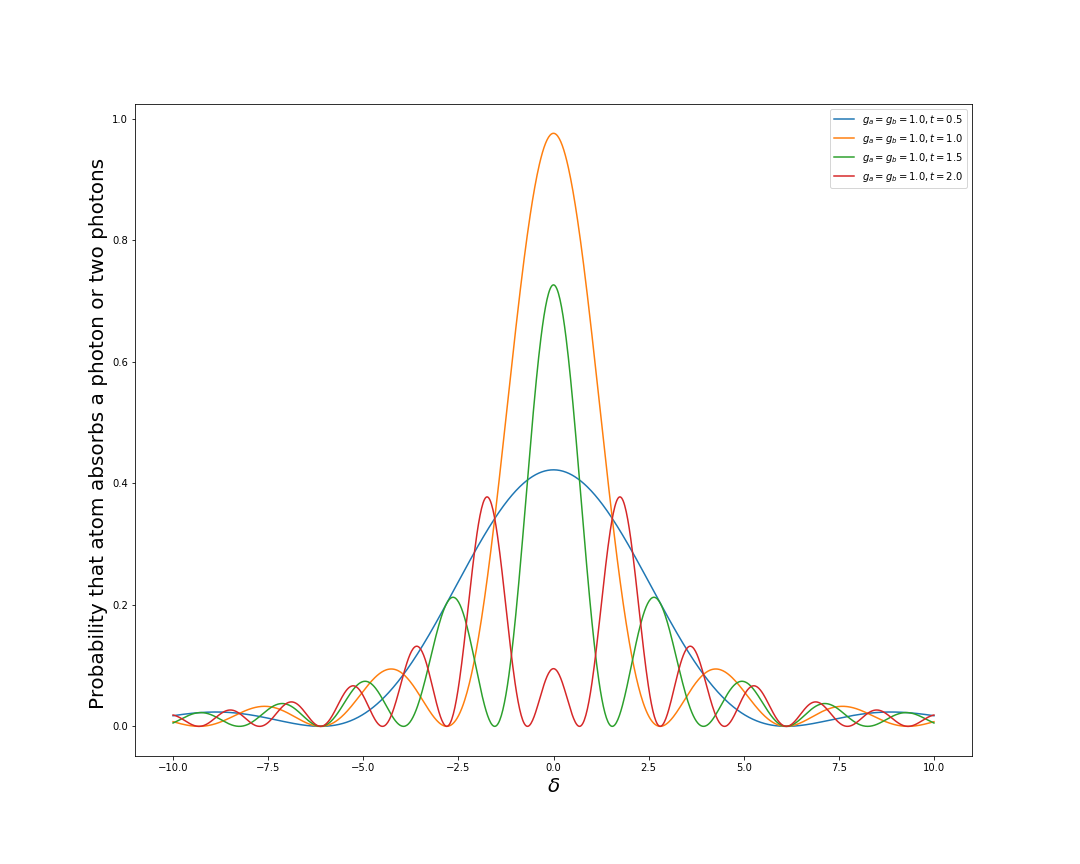
\includegraphics[width = 100mm]{../fig/ex7_22.png}
        \end{center}
    \end{figure}
\end{ex}

\begin{ex}
    \label{ex7.23}
\end{ex}